\documentclass{beamer}

\usetheme{CambridgeUS}
\usecolortheme{orchid}

\usepackage[utf8]{inputenc}
\usepackage[T1]{fontenc}

% Math
\usepackage{amsmath}
\usepackage{amssymb}
\usepackage{bm}

% Graphics
\usepackage{graphicx}
\usepackage{caption}
\usepackage{subcaption}
\graphicspath{{../figs/}}

% Colors
\definecolor{darkblue}{HTML}{00688B}
\definecolor{darkgreen}{HTML}{6E8B3D}
\definecolor{cadet}{HTML}{DAE1FF}
\definecolor{salmon}{HTML}{FFB08A}

% Listings
\usepackage{textcomp}
\usepackage{listings}
\lstset{
  keywordstyle=\bfseries\color{orange},
  stringstyle=\color{darkblue!80},
  commentstyle=\color{darkblue!80},
  showstringspaces=false,
  basicstyle=\ttfamily,
  upquote=true,
}
\lstdefinestyle{fortran}{
  language=Fortran,
  morekeywords={for},
  deletekeywords={status},
}
\lstdefinestyle{c}{
  language=C,
  morekeywords={include},
}
\lstdefinestyle{shell}{
  language=bash,
}

\subtitle{TMA4280---Introduction to Supercomputing}

\begin{document}


\title{Message passing and MPI}
\author{Eivind Fonn}
\institute{SINTEF ICT / NTNU}
\date{December 2015}
\maketitle

\begin{frame}
  \frametitle{The message passing model}
  \begin{center}
    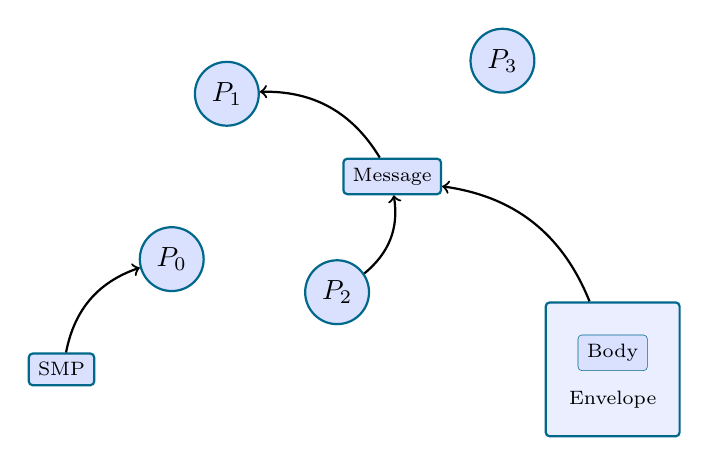
\begin{tikzpicture}[
  proc/.style={shape=circle, draw=darkblue, fill=cadet, thick},
  msg/.style={shape=rectangle, draw=darkblue, fill=cadet, thick, rounded corners=0.5mm},
  env/.style={minimum height=1.7cm, minimum width=1.7cm},
  scale=0.7,
  ]
  \node[proc] (p0) at (0,0) {$P_0$};
  \node[proc] (p1) at (1,3) {$P_1$};
  \node[proc] (p2) at (3,-0.6) {$P_2$};
  \node[proc] (p3) at (6,3.6) {$P_3$};
  \node[msg] (msg) at (4.0, 1.5) {\scriptsize Message};
  \node[msg, env, fill=cadet!55] (env) at (8, -2.0) {};
  \node[msg, very thin] (body) at (8, -1.7) {\scriptsize Body};
  \node[below of=body, node distance=6mm] {\scriptsize Envelope};
  \draw[->, thick] (p2) edge[bend right] node [right] {} (msg);
  \draw[->, thick] (msg) edge[bend right] node [right] {} (p1);
  \draw[->, thick] (env) edge[bend right] node [right] {} (msg);

  \node[msg] (smp) at (-2,-2) {\scriptsize SMP};
  \draw[->, thick] (smp) edge[bend left] node [right] {} (p0);
\end{tikzpicture}

  \end{center}
\end{frame}

\begin{frame}[fragile]
  \frametitle{MPI with C}
  \scalebox{0.5}{
    \lstinputlisting[style=c]{\code/mpi_hello/c/hello.c}
  }
\end{frame}

\begin{frame}[fragile]
  \frametitle{MPI with Fortran}
  \scalebox{0.5}{
    \lstinputlisting[style=fortran]{\code/mpi_hello/fortran/hello.f90}
  }
\end{frame}

\begin{frame}[fragile]
  \frametitle{Sample output with four processors}
  \begin{center}
    \begin{tabular}{c}
\begin{lstlisting}
Process 0: Hello, world!
Process 1: Hello, world!
Process 3: Hello, world!
Process 2: Hello, world!
\end{lstlisting}
    \end{tabular}
  \end{center}
  Note that ordering is not guaranteed.
\end{frame}

\begin{frame}
  \frametitle{MPI: Message Passing Interface}
  Advantages of the MPI message-passing model:
  \begin{itemize}
  \item standardization;
  \item portability;
  \item performance;
  \item expressiveness.
  \end{itemize}

  MPI is a library comprising about 125 functions or operations:
  \begin{itemize}
  \item \textcolor{red}{one-to-one} operations (or point-to-point communication);
  \item \textcolor{red}{one-to-all} operations;
  \item \textcolor{red}{all-to-one} operations;
  \item \textcolor{red}{all-to-all} operations.
  \end{itemize}
  The last three types are referred to as {\em collective} operations.
\end{frame}

\input{postamble}
